\chapter{Bootstrapping Process}
\label{process}

This chapter describes the bootstrapping process in its entirety.
The entire process can be divided into three phases.
During the bootstrapping phase, the local and remote bootware components are started and provision a provisioning engine, which in turn provisions the workflow middleware.
Once the workflow middleware is ready, the second phase starts, which is the workflow execution phase.
During this phase, the remote bootware might be called multiple times to deploy or undeploy new provisioning engines.
The third and final phase, the shutdown phase, begins when the workflow execution is finished.
In this phase, all remaining services, provisioning engines, the workflow middleware, the remote and the local bootware, as well as all the underlying infrastructure are deprovisioned.
In \autoref{image:process}, we can see the whole process with numerated steps.
We will go through \autoref{image:process} step by step in the following paragraphs to get a better understanding of the whole bootstrapping process.

\begin{figure}[!htbp]
	\centering
	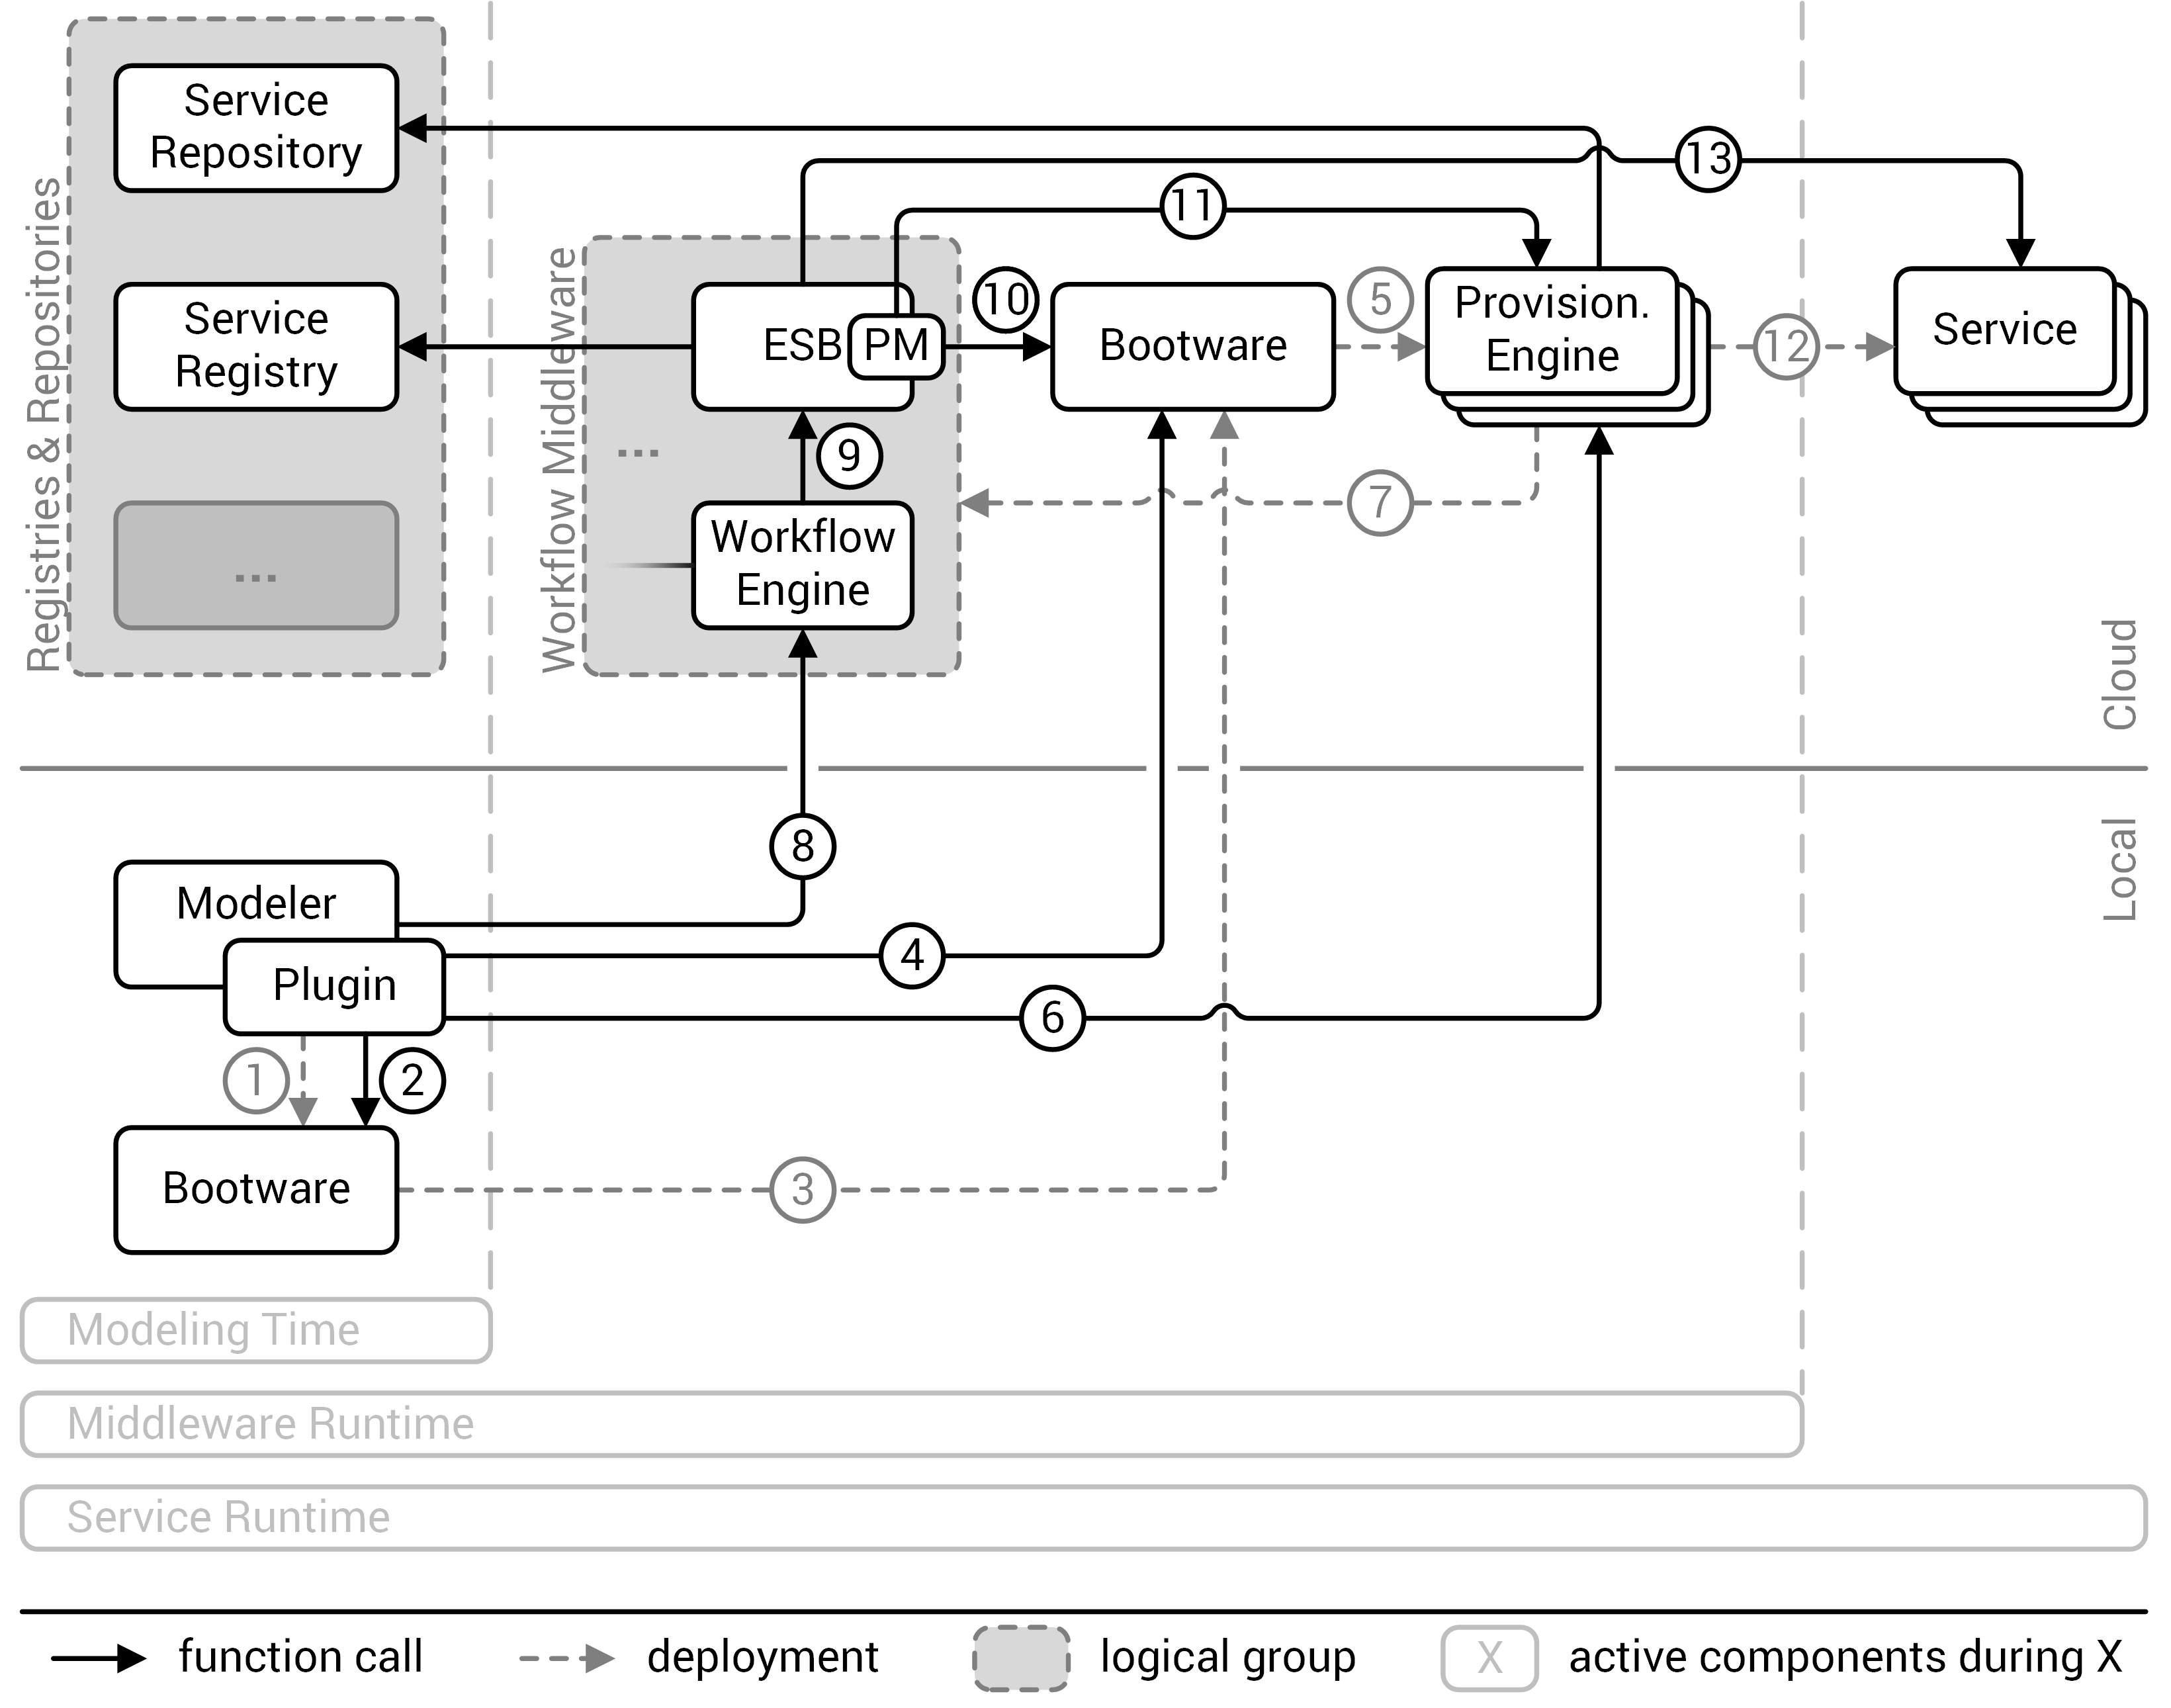
\includegraphics[resolution=600]{process/assets/process}
	\caption{The step-by-step bootware process.}
	\label{image:process}
\end{figure}

At the beginning, a user starts the Modeler, which includes the bootware adapter, as seen on the bottom left of \autoref{image:process}.
If they have not done so already, they configure the bootware adapter with their cloud login credentials to be used during the bootware process and other parameters that might be needed. They also select, which event plugins the bootware should load.
They then use the Modeler to create a workflow as usual.
Once the workflow is finished and ready to be executed, they click the start button as usual.
This marks the beginning of the bootstrapping phase.
The bootware adapter has hooked into the start process and takes over by starting the local bootware (step 1).

Once the local bootware is up and running, the bootware adapter calls it with the context the user provided (step 2).
The local bootware first checks, if a remote bootware already exists in the requested remote environment.
If not, the local bootware provisions a remote bootware using the information provided in the context (step 3).
Once the remote bootware is deployed, it is called by the local bootware with a deploy request for the provisioning engine that will be used to deploy the workflow middleware (step 4).
The remote bootware deploys the requested provisioning engine using the information provided in the context (step 5).
Once the provisioning engine is up and running, the remote bootware calls the provisioning engine (step 6) and tells it to deploy the workflow middleware (step 7).
Once the workflow middleware is up and running, the provisioning engine returns the endpoint references of the workflow middleware to the remote bootware, which in turn returns it to the local bootware, which returns it to the bootware adapter.
The bootware adapter uses those end point references to link the modeler to the workflow middleware.
This is the end of the bootstrapping phase.
Now begins the workflow execution phase.

Once linked, the modeler deploys the workflow on the workflow middleware as usual and starts its execution (step 8).
The workflow middleware now executes the workflow, during which it might encounter a point where it has to call a remote service.
The remote service call is passed on to the ESB (step 9), which checks if the service is already reachable.
If it is, execution continues as usual.
If not, the ESB tells the provisioning manager to provision the requested service (step 10).
The provisioning manager checks if the provisioning engine needed to provision the requested service is already available.
If it is not, the provisioning manager calls the remote bootware with a request to provision the required provisioning engine (step 11).
The remote bootware provisions the provisioning engine using the information from the request and the user context (step 5).
Once the provisioning engine is up and running, the remote bootware returns the endpoint reference of the provisioning engine to the provisioning manager.
The provisioning manager now calls the provisioning engine (step 12) and tells it to provision the required service (step 13).
Once the service is available, the provisioning engine returns its endpoint reference to the provisioning manager, who in turn returns it to the ESB.
The ESB can now call the service (step 14) and use the service response to continue with the workflow execution.
The workflow execution now continues in this fashion, spawning new provisioning engines and services through the provisioning manager and the remote bootware along the way (repeating steps 9, 10, 11, 5, 12, 13 and 14).
At some point, the workflow will be finished.
This marks the end of the workflow execution phase and the start of the shutdown phase.

If it has not done so already, the provisioning manager calls all relevant provisioning engines to undeploy any services that might still be running (step 12, 13).
Once all services are undeployed, the work of the workflow middleware is finished.
The bootware is listening at the workflow middleware for this event and triggers the undeploy process once it happens.
First, the remote bootware calls the provisioning engine that was used to provision the workflow middleware (step 6) and tells it to undeploy the workflow middleware (step 7).
The provisioning engine returns the success to the remote bootware.
Next, the remote bootware undeploys all provisioning engines that might still be running (step 5).
Once all provisioning engines are gone, the remote bootware returns the success to the local bootware.
The local bootware removes the remote bootware (step 3) and returns the success to the bootware adapter.
At this point, no remote components should be running anymore.
The local bootware now shuts down itself, which completes the whole process.

\autoref{image:startup_sequence} shows the bootstrapping phase as sequence diagram, which displays the interaction between the components arranged by time from top to bottom.
The lifetime of a particular component is represented by a dashed line running from the top to the bottom.
If an activity box is displayed over the line, the component is active at this moment in time.
Activity is usually triggered by receiving a call from another component and ended by returning a response to this call.
Calls are represented by arrows between activity boxes.
The can be further distinguished between synchronous and asynchronous calls, depending on the form of the arrow head.
A response is displayed as a dashed arrow between activity boxes.
The end of the lifetime of a component (i.e. when it is shutdown) is marked by a cross that ends the lifetime line.

\begin{figure}[!htbp]
	\centering
	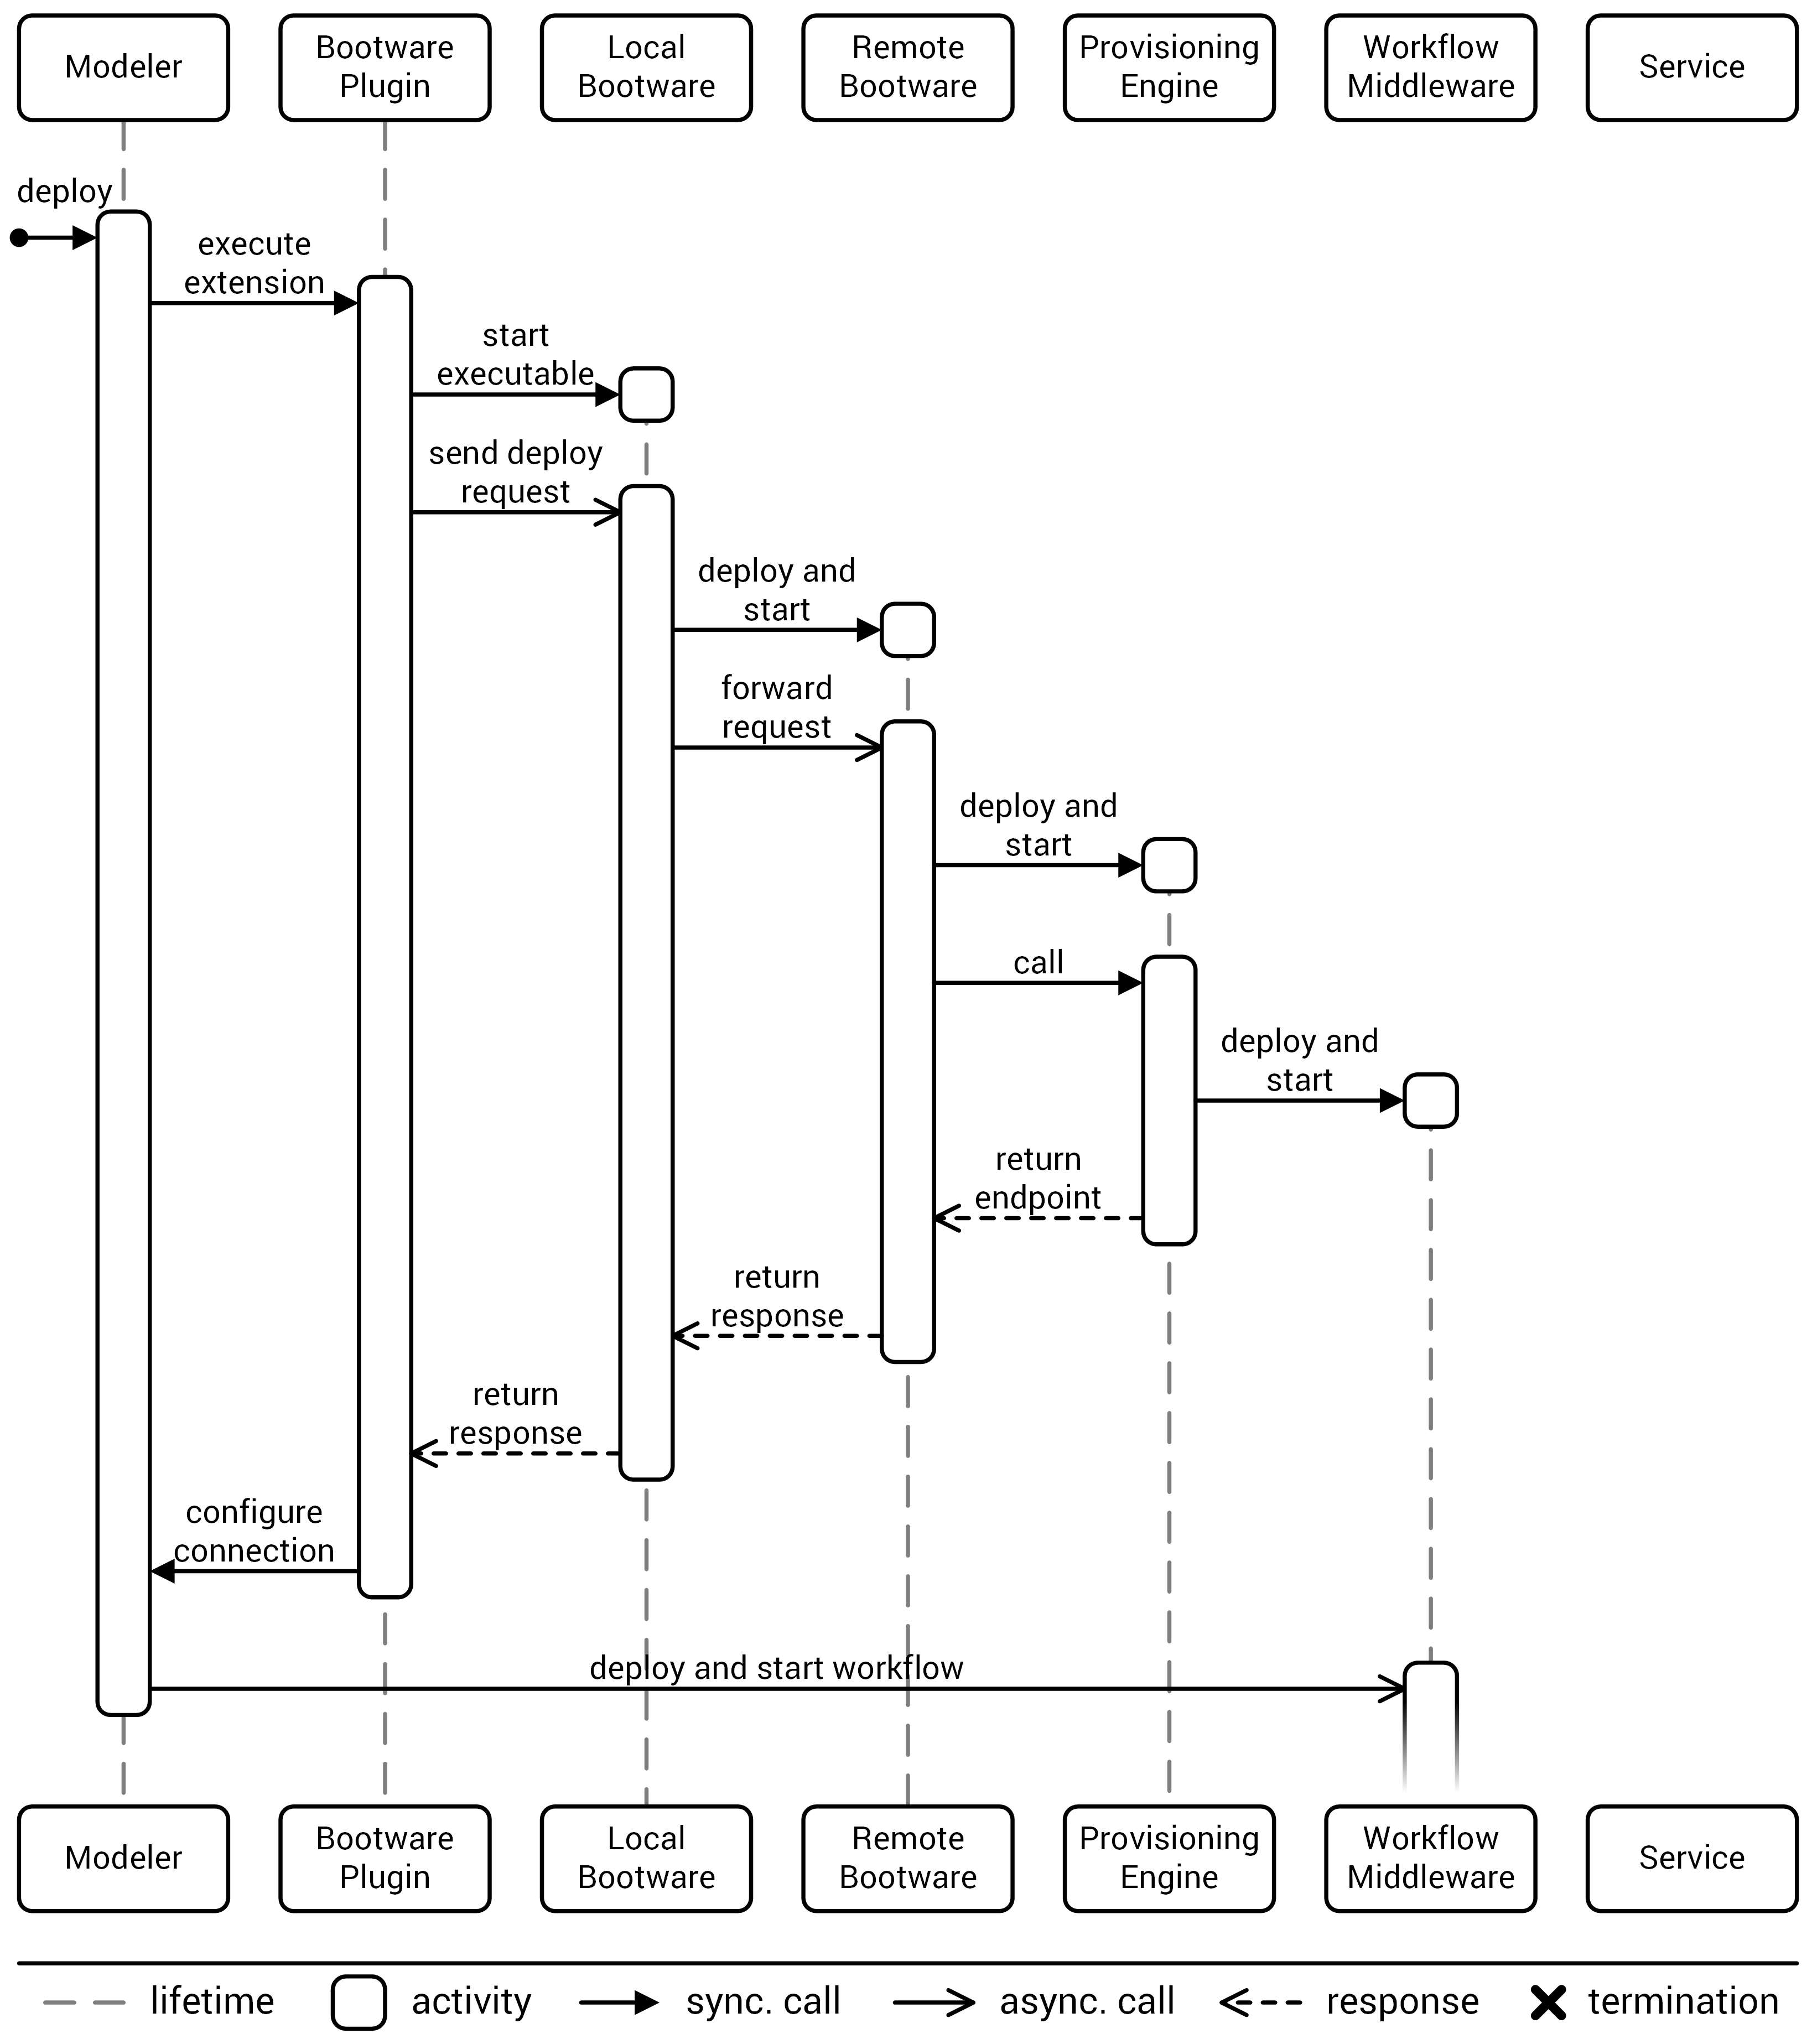
\includegraphics[resolution=600]{process/assets/bootstrapping_sequence}
	\caption{Sequence diagram of the bootstrapping phase.}
	\label{image:startup_sequence}
\end{figure}

In \autoref{image:startup_sequence} we can clearly see how one component triggers the next one during the bootstrapping phase.
Starting at the top left, the deploy action starts an escalating process, where one component starts the next, beginning with the modeler starting the bootware adapter.
The bootware adapter then starts the local bootware and sends a deploy requests.
The local bootware deploys and starts the remote bootware and forwards the deploy request.
The remote bootware deploys and starts a provisioning engine, which it then calls to provision the workflow middleware.
Once the workflow middleware is running, every component returns a response to the component who called it, which ends when the bootware adapter receives a response from the local bootware.
This response contains the endpoint references to the workflow middleware, which the bootware adapter uses to configure the connection between the modeler and the workflow middleware.
The modeler can now deploy and start the workflow on the workflow middleware, which concludes the bootstrapping phase.

\begin{figure}[!htbp]
	\centering
	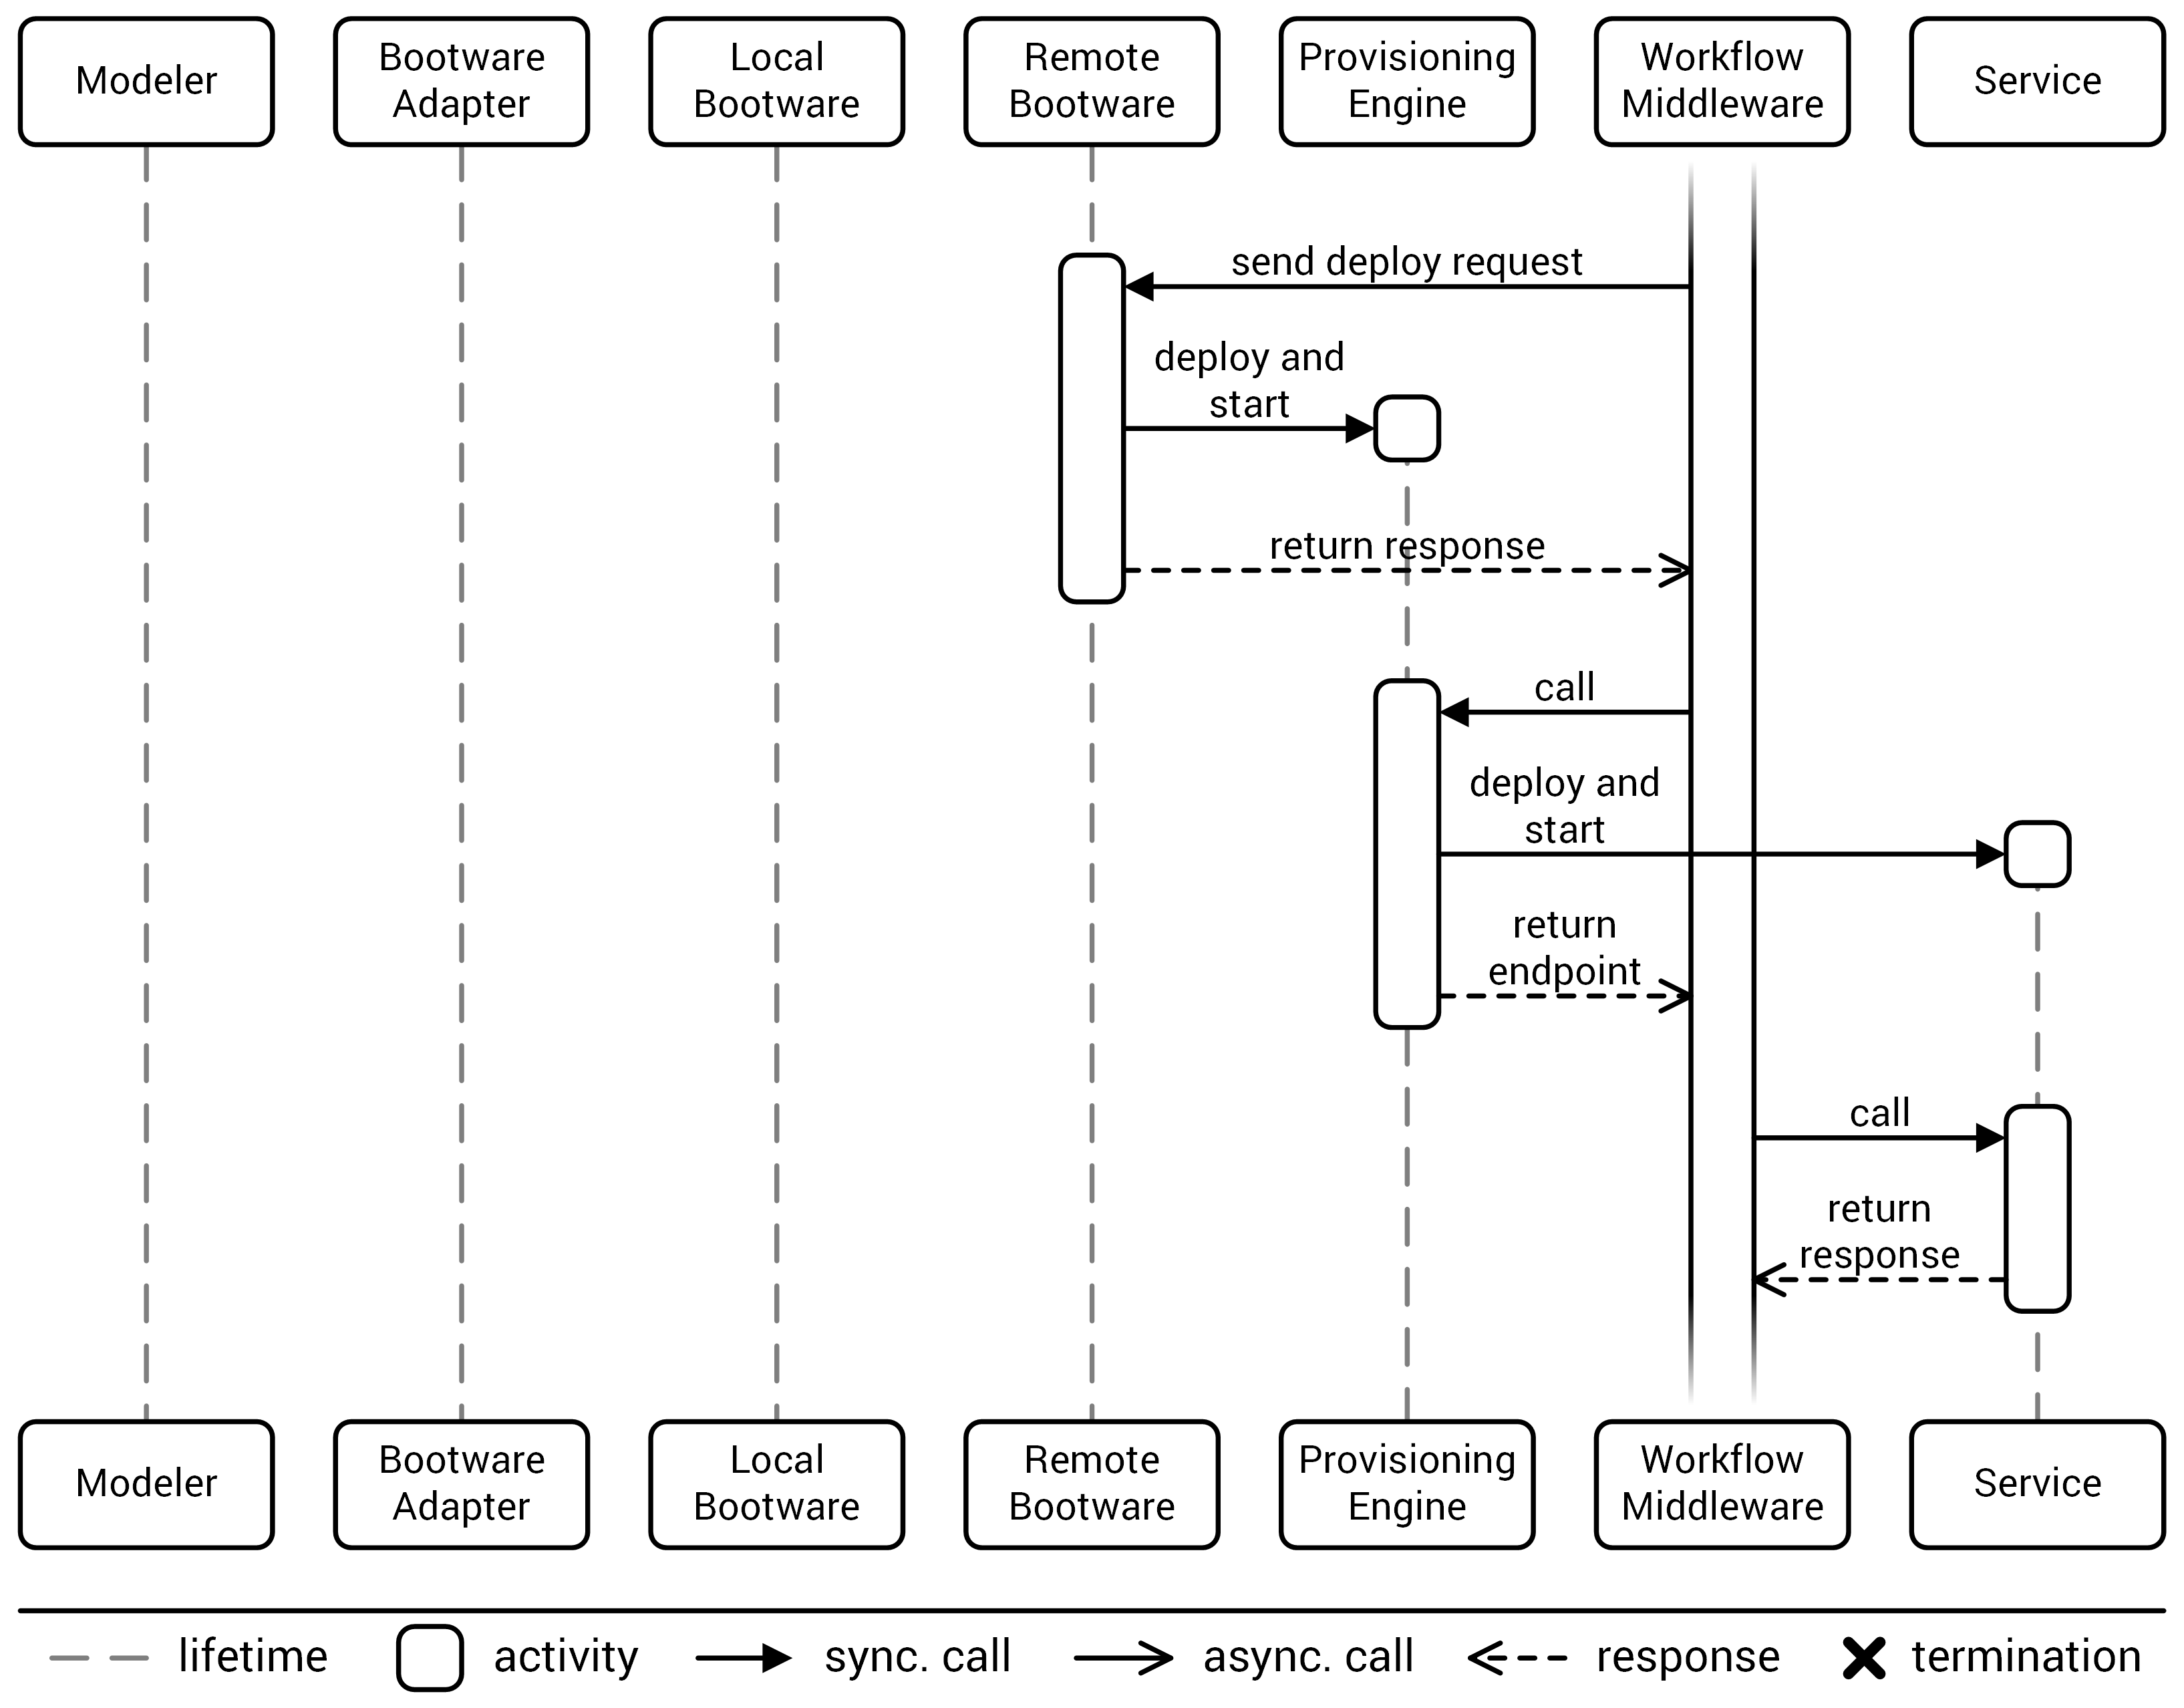
\includegraphics[resolution=600]{process/assets/workflow_execution_sequence}
	\caption{Sequence diagram of the workflow execution phase.}
	\label{image:execution_sequence}
\end{figure}

In the workflow execution phase, which is also depicted as a sequence diagram in \autoref{image:execution_sequence}, the workflow middleware might now call external services.
If these services do not exist already, the workflow middleware has to provision them first (via the provisioning manager).
To provision a service, a particular provisioning engine is needed, which also might not exist yet.
In this case, a deploy request is send from the workflow middleware (i.e. the provisioning manager) to the remote bootware, which then deploys and starts the requested provisioning engine.
Once the particular provisioning engine exists, the workflow middleware calls it to deploy the service it wants to execute.
This process might be repeated multiple times during the whole workflow execution.

\begin{figure}[!htbp]
	\centering
	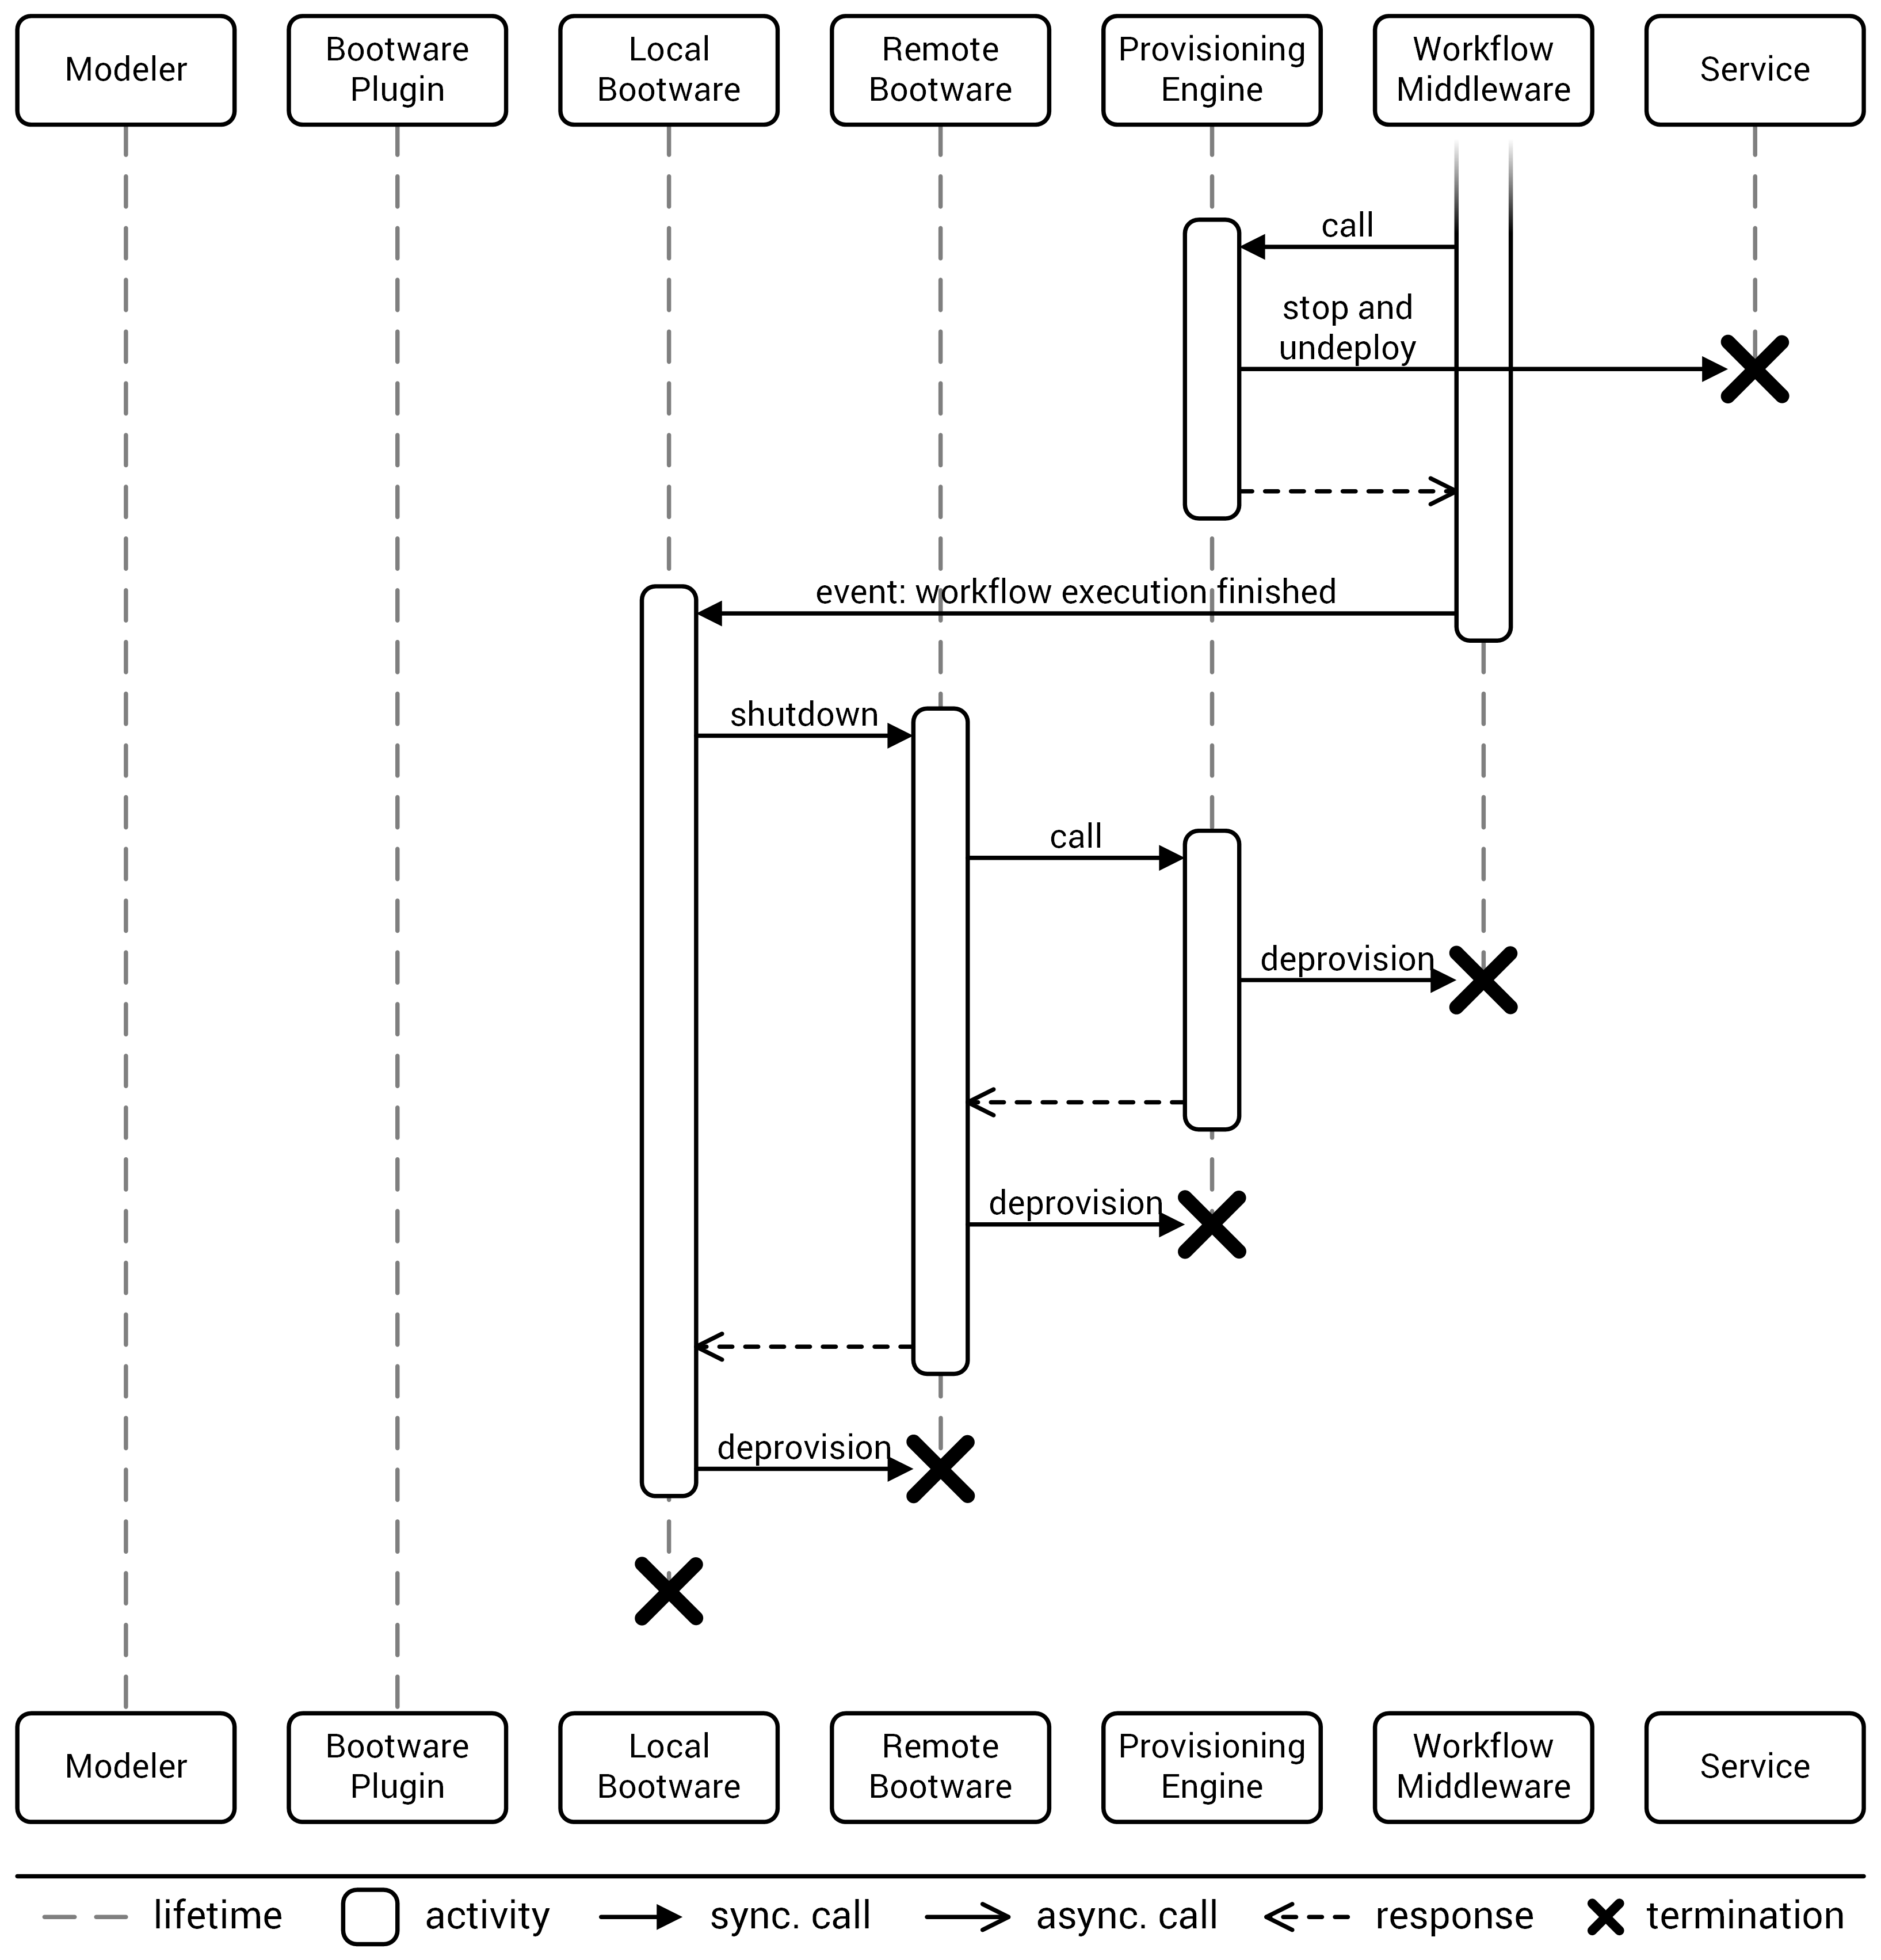
\includegraphics[resolution=600]{process/assets/shutdown_sequence}
	\caption{Sequence diagram of the shutdown phase.}
	\label{image:shutdown_sequence}
\end{figure}

The shutdown phase begins once the workflow execution is finished.
As we can see in \autoref{image:shutdown_sequence}, the workflow might need to stop and undeploy remaining services by calling the particular provisioning engines via the provisioning manager.
Once all services are removed, the workflow execution is truly finished and an event marking this state is emitted.
The local bootware has been listening for this event through one of its event plugins and triggers the removal of the remaining components by first calling the shutdown operation of the remote bootware.
The remote bootware calls a provisioning engine to deprovision the workflow middleware, before deprovisioning all remaining provisioning engines itself.
Once this is done, a response is send to the local bootware, which can now deprovision the remote bootware, before shutting down itself.
This concludes the shutdown phase and the whole bootware process.
